\documentclass[10pt]{beamer}
\geometry{paperwidth=16cm, paperheight=12cm} % 设置页面宽度为16厘米,高度为12厘米
%\setlength{\parindent}{1em} % 设置首行缩进为1个字符的宽度

\setbeamertemplate{caption}[numbered]  % 设置图表编号
\setbeamertemplate{bibliography item}[text]  % 设置参考文献项目样式
\useinnertheme{circles}
\usepackage{tikz}
\usepackage{geometry}
% \usepackage{titlesec}
% \usepackage{titletoc}
\usepackage{caption}
\usepackage{hyperref}
\usepackage{listings}
\usepackage{hyperref}
\usepackage{xcolor}
\usepackage{siunitx}
\usepackage{perpage}
\usepackage{amsmath}
\usepackage{fancyhdr}

\usepackage[UTF8]{ctex}
\usepackage{fontspec}

\captionsetup[figure]{skip=0pt}
\captionsetup[table]{skip=0pt}

% 设置文档的默认字体为华文仿宋


\mode<presentation> {
	\usetheme{Frankfurt}  % 使用Frankfurt主题
	\usefonttheme{serif}
	% 自定义柔和的颜色主题
	\definecolor{SoftBlue}{RGB}{70,130,180} % 柔和的蓝色
	\definecolor{SoftGray}{RGB}{240,240,240} % 柔和的灰色
	
	% 设置主要元素的颜色
	\setbeamercolor{palette primary}{bg=SoftBlue, fg=white}
	\setbeamercolor{palette secondary}{bg=SoftBlue!70, fg=white}
	\setbeamercolor{palette tertiary}{bg=SoftBlue!60, fg=white}
	\setbeamercolor{palette quaternary}{bg=SoftBlue!50, fg=white}
	
	% 设置顶部导航栏和页脚的颜色
	\setbeamercolor{section in head/foot}{bg=SoftGray, fg=black}
	\setbeamercolor{footline}{bg=SoftBlue, fg=white}
	
	% 设置标题和帧标题的颜色
	\setbeamercolor{title}{bg=SoftBlue, fg=white}
	\setbeamercolor{frametitle}{bg=SoftBlue, fg=white}
	
	% 设置目录和列表项的颜色
	\setbeamercolor{section in toc}{fg=SoftBlue}
	\setbeamercolor{itemize item}{fg=SoftBlue}
	\setbeamercolor{itemize subitem}{fg=SoftBlue}
	\setbeamercolor{itemize subsubitem}{fg=SoftBlue}
	\setbeamercolor{enumerate item}{fg=SoftBlue}
	
	% 设置块标题的颜色
	\setbeamercolor{block title}{bg=SoftBlue, fg=white}
	\setbeamercolor*{block title example}{bg=white, fg=SoftBlue}
	% 幻灯片的标题字体大小 大号并加粗
	\setbeamerfont{frametitle}{size={\Large }, series=\bfseries}
	
	% 设置幻灯片编号样式
	\setbeamertemplate{footline}[frame number]
	% 使用圆形项目符号
%	\useinnertheme{circles}
	% 设置边栏颜色
	\setbeamercolor{sidebar}{bg=SoftBlue}
	% 设置其他元素的颜色
	\setbeamercolor{structure}{fg=SoftBlue}
	% 取消注释此行以在所有幻灯片中移除脚部线
	\setbeamertemplate{footline} 
	% 取消注释此行以用简单的幻灯片计数替换所有幻灯片中的脚部线
	%\setbeamertemplate{footline}[page number] 
	 % 取消注释此行以从所有幻灯片底部移除导航符号
	%\setbeamertemplate{navigation symbols}{}
}



%\usepackage[UTF8]{ctex}
%\setCJKmainfont{Microsoft YaHei} % 全局设置正文字体为微软雅黑

\usepackage{
	hyperref,   % 可点击的链接
	graphicx,   % 包含图像
	listings,   % 代码和格式化
%	caption,    % 图表和表格的标题自定义
	stackengine,% 自定义布局
	amsmath,    % 数学环境
	xcolor,     % 扩展颜色支持
	multicol,   % 多列布局
	booktabs,   % 表格
	bookman,    % 使用的字体
	graphicx,   % 允许包含图像
	booktabs,   % 允许使用表格中的 \toprule, \midrule 和 \bottomrule
	ctex,       % 支持中文
	lipsum, 		% remove it
}
\usepackage{changepage}
\usepackage{listings}

\definecolor{codered}{rgb}{0.6,0,0}
\definecolor{codeblue}{rgb}{0,0,0.8}
\definecolor{codegreen}{rgb}{0,0.5,0}
\definecolor{almostwhite}{gray}{0.55}
\definecolor{codepurple}{rgb}{0.58,0,0.82}
\definecolor{backcolour}{rgb}{0.95,0.95,0.92}

\lstset{
	language=Python,                 % 设置语言
	basicstyle=\ttfamily\small,      % 设置代码字体和大小:等宽字体、小号字体
	keywordstyle=\bfseries\color{codeblue},       % 设置关键字颜色:加粗、蓝色
	emphstyle=\ttfamily\color{codered},    % 自定义高亮样式:等宽字体、红色
	stringstyle=\color{codepurple},        % 设置字符串的样式:紫色
	numbers=none,                          % 在左侧显示行号
	breaklines=true,                 % 自动换行
	showstringspaces=false,          % 不显示字符串中的空格
	showtabs=false ,                  % 来隐藏Tab键的表示
	numberstyle=\small\color{almostwhite}, % 设置行号的样式:小号字体、接近白色
	rulesepcolor=\color{red!20!green!20!blue!20}, % 设置代码框分隔线的颜色:混合红绿蓝
	frame=shadowbox,                       % 设置代码框的样式:阴影框
	commentstyle=\color{codegreen},        % 设置注释的样式:绿色
	captionpos=b                       % 设置标题位置:底部('b' stands for 'bottom')
}


%	标题页
\title[]{ {\Large 基于决策树模型和神经网络模型的降雨量问题研究 }}
%\subtitle{一个简短的故事}
%作者
\author[Arthur, Doe]{\textbf{李沐阳 \and 钟绍恒 \and 易领程}}
%作者详情
\institute[VFU] {}

\date{\today} % 自动插入当前日期


%----------------------------------------------------------------------------------------
%	当前章节的标题高亮
%----------------------------------------------------------------------------------------
\AtBeginSection[]
{
	\begin{frame}
		\frametitle{目录}
		\tableofcontents[currentsection]
	\end{frame}
}

% 插入代码 \lstinputlisting{code.py}

%	\begin{frame}
%	\frametitle{样本帧标题}
%	\alert{高亮} 
%	\begin{block}{备注}
%		样本文本
%	\end{block}
%	
%	\begin{alertblock}{重要定理}
%		红色框中的样本文本
%	\end{alertblock}
%	
%	\begin{examples}
%		绿色框中的样本文本。块的标题是``例子"。
%	\end{examples}
%\end{frame}

% 两栏
%\begin{columns}
%% 插入一个带有两列的样本帧 --------------------------------
%
%\column{0.5\textwidth}
%这是第一列中的文本。
%$$E=mc^2$$
%\begin{itemize}
%	\item 第一项
%	\item 第二项
%\end{itemize}
%
%\column{0.5\textwidth}
%这段文本将出现在第二列中
%并且在某些情况下,这是一个不错的布局。
%\end{columns}




\begin{document}
{
% Remove headline and footline from first slide
\setbeamertemplate{footline}{}
\setbeamertemplate{headline}{}
% 插入标题页---------------------------
\frame{\titlepage}
}


%插入目录------------------------------



\begin{frame}
	\frametitle{基于决策树模型和神经网络模型的降雨量问题研究}


	\begin{description}
		\item[论文标题:]  基于决策树模型和神经网络模型的降雨量问题研究
		      % \item[论文链接:]   \url{https://doi.org/10.48550/arXiv.2401.00423}
		\item[代码链接:]   \url{https://github.com/limuy2022/math_model}
		\item[发表年份:]   2024
		      % \item[发表平台:]  AAAI
		      % \item[平台等级:]  CCF A
		\item[作者信息:]   李沐阳$^1$ ,钟绍恒$^2$ , 易领程$^3$

		      \begin{enumerate}
			      \item  东莞市东华高级中学120班学生
			      \item 	 东莞市东华高级中学120班学生
			      \item 	 东莞市东华高级中学120班学生
		      \end{enumerate}
	\end{description}

\end{frame}

\section{研究背景与前提假设}
\begin{frame}
	\frametitle{研究背景}
	\begin{block}{研究背景}
		现如今, 气候无不影响着人类的生活, 探寻其中各种因素的关系成为了当务之急.
		在此前提下, 我们决定着手降水量的研究, 试图为气象研究提供参考.
		考虑到现实因素的复杂性, 我们决定简化问题,将其转化为$5$个自变量和
		$1$个因变量之间的函数关系.
		本篇论文主要研究欧洲``降水量``与``气温``、``海平面气压``、 ``风
		速``、``湿度``、``云层覆盖``之间的关系.
		同时, 为了方便表达, 我们规定了一下符号以及其中的单位,如下表所示:
	\end{block}
	\begin{block}{符号说明}
		\begin{table}[h!]
			\centering
			\caption{符号说明}
			\begin{tabular}{p{6em}p{6em}l}
				\hline
				符号  & 说明   & 单位                          \\
				\hline
				$r$ & 降雨量  & \si{\milli\meter}           \\
				$t$ & 温度   & $0.1$\si{\degreeCelsius}    \\
				$f$ & 风速   & $0.1$\si{\meter\per\second} \\
				$h$ & 湿度   & $0.1\%$                     \\
				$c$ & 云层覆盖 & \si{octas}                  \\
				$p$ & 气压   & $0.1$\si{h\pascal}          \\
				\hline
			\end{tabular}
		\end{table}
	\end{block}
\end{frame}

\begin{frame}
	\frametitle{前提假设}
	\begin{block}{前提假设}
		\begin{itemize}
			\item 排除一切人为影响气候因素, 如工业排放, 热岛效应等.
			\item 排除次要因素对降水量的影响, 如辐射、空气污染等.
			\item 假设降水量只与气温、气压、风速、湿度、云层覆盖有关.
			\item 降水量准确的标准为:得出的降水量$r$和正确的降水量$r_0$满足关系$r_0 - 10 \le r \le r_0 + 10$.
		\end{itemize}
	\end{block}
\end{frame}

\section{模型尝试}
\subsection{线性回归模型}
\begin{frame}
	\frametitle{线性回归模型}
	\begin{block}{模型假设}
		\begin{itemize}
			\item 降水量与气温、气压、风速、湿度、云层覆盖之间存在线性关系.
			\item 线性关系式导致的误差可忽略.
			      % \item 线性关系中的截距项为$0$.
		\end{itemize}
	\end{block}

	\begin{block}{研究方法}
		考虑到拟合线性关系, 我们决定采用较为常见的最小二乘法进行模型拟合.
	\end{block}
\end{frame}

\begin{frame}
	\frametitle{最小二乘法简介}
	\begin{block}{基本概念}
		最小二乘法是一种求解线性方程组的方法, 该方法的基本思想是将
		线性方程组表示为如下形式的最小二乘方程组:
		\begin{equation}
			% \begin{cases}
			y = \beta_0 + \beta_1 x_1 + \beta_2 x_2 + \beta_3 x_3 + \beta_4 x_4 + \beta_5 x_5
			% \end{cases}
		\end{equation}
		其中$x_1$、$x_2$、$x_3$、$x_4$、$x_5$分别代表云层覆盖、湿度、气温、气压、风速.
	\end{block}
	\begin{block}{求解公式}
		最小二乘法的求解公式如下所示:
		\begin{equation}
			\begin{cases}
				% \bar{y} = \beta_0 + \beta_1 \bar{x_1} + \beta_2 \bar{x_2} + \beta_3 \bar{x_3} + \beta_4 \bar{x_4} + \beta_5 \bar{x_5} \\
				\beta_0 = \bar{y} - \beta_1 \bar{x_1} - \beta_2 \bar{x_2} - \beta_3 \bar{x_3} - \beta_4 \bar{x_4} - \beta_5 \bar{x_5} \\
				\beta_1 = \frac{\sum_{i=1}^n (x_{1_i} - \bar{x_1}) (y_i - \bar{y})}{\sum_{i=1}^n (x_{1_i} - \bar{x_1})^2}             \\
				\beta_2 = \frac{\sum_{i=1}^n (x_{2_i} - \bar{x_2}) (y_i - \bar{y})}{\sum_{i=1}^n (x_{2_i} - \bar{x_2})^2}             \\
				\beta_3 = \frac{\sum_{i=1}^n (x_{3_i} - \bar{x_3}) (y_i - \bar{y})}{\sum_{i=1}^n (x_{3_i} - \bar{x_3})^2}             \\
				\beta_4 = \frac{\sum_{i=1}^n (x_{4_i} - \bar{x_4}) (y_i - \bar{y})}{\sum_{i=1}^n (x_{4_i} - \bar{x_4})^2}             \\
				\beta_5 = \frac{\sum_{i=1}^n (x_{5_i} - \bar{x_5}) (y_i - \bar{y})}{\sum_{i=1}^n (x_{5_i} - \bar{x_5})^2}             \\
			\end{cases}
		\end{equation}
		其中$\bar{y}$、$\bar{x_1}$、$\bar{x_2}$、$\bar{x_3}$、$\bar{x_4}$、$\bar{x_5}$分别代表
		降水量的均值、云层覆盖的均值、湿度的均值、气温的均值、气压的均值、风速的均值.
	\end{block}
\end{frame}

\begin{frame}
	\frametitle{最小二乘法结果}
	\begin{block}{结果展示}
		最小二乘法的求解结果如下所示:
		% \begin{align}
		% 	\notag
		% 	r & =315.80363888548624+6.197181723408759c+0.15411116711110595h \\
		% 	\notag
		% 	  & \qquad +0.16901104754961455t-0.03432027705042855p+0.17773547386441546f
		% \end{align}
		\begin{equation}
			\begin{cases}
				\beta_0 = 315.80363888548624   \\
				\beta_1 = 6.197181723408759    \\
				\beta_2 = 0.15411116711110595  \\
				\beta_3 = 0.16901104754961455  \\
				\beta_4 = -0.03432027705042855 \\
				\beta_5 = 0.17773547386441546
			\end{cases}
		\end{equation}
	\end{block}
	\begin{block}{模型误差}
		正确率为$60\%$左右,最小二乘法的拟合图像如下所示:
		\begin{figure}[h!]
			\centering
			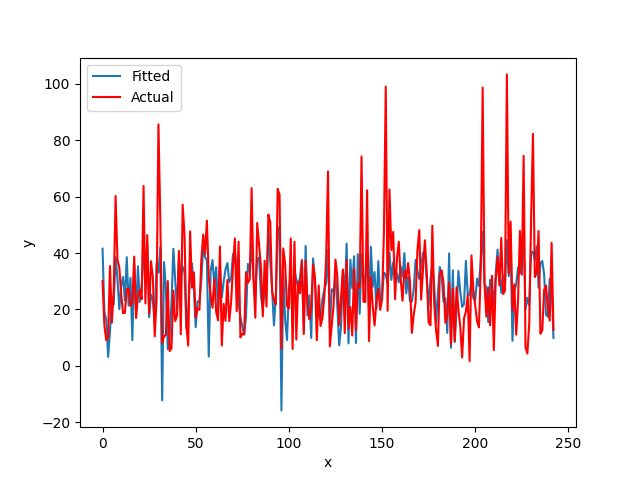
\includegraphics[scale=0.2]{../src/try_match/ols_five.png}
			\caption{拟合降水量和真实降水量的折线统计图}
		\end{figure}
	\end{block}
\end{frame}

\subsection{神经网络}
\begin{frame}
	\frametitle{神经网络}
	\begin{block}{网络规模}
		本网络采用的规模为$5 \times 64 \times 64 \times 64 \times 64 \times 1$的全连接神经网络$^1$.
		其中, 第$1$层为输入的五个自变量, 第$6$层的值为降水量的预测值.
		神经元采用的激活函数为Leaky ReLU函数$^2$.
		\begin{enumerate}
			\item 全连接神经网络(Fully Connected Neural Network,简称FCNN)是一种最基础的人工神经网络结构,也称
			      为多层感知器(Multilayer Perceptron,MLP)
			\item 函数表达式为:$f(x)=\max(0, x) + \alpha \cdot \min(0, x)$
		\end{enumerate}
	\end{block}
\end{frame}

\end{document}<ScrollWheelUp>
